\section{Quaternions}\label{sec:quaternions}

A quaternion $q\in\mathbb{H}$ takes the form
$q =  a\boldsymbol{1} + b\boldsymbol{i} + c\boldsymbol{j} + d\boldsymbol{k}$,
where $(a,b,c,d) \in \R^4$, and $\boldsymbol{1}$, $\boldsymbol{i}$, $\boldsymbol{j}$, and $\boldsymbol{k}$ are the fundamental quaternion units
\begin{equation*}
    \boldsymbol{1} = \begin{pmatrix} 1 & 0 \\ 0 & 1 \end{pmatrix}, \quad
    \boldsymbol{i} = \begin{pmatrix} i & 0 \\ 0 & -i \end{pmatrix}, \quad
    \boldsymbol{j} = \begin{pmatrix} 0 & 1 \\ -1 & 0 \end{pmatrix}, \quad
    \boldsymbol{k} = \begin{pmatrix} 0 & i \\ i & 0 \end{pmatrix},
\end{equation*}
with $i$ the imaginary unit.
Any quaternion $q$ can thus be represented by its set of coefficients $(a,b,c,d)\in\mathbb{R}^4$.
The algebra $\mathbb{H}$ is similar to the algebra of complex numbers $\mathbb{C}$, with the exception of the multiplication operation being non-commutative.

Unit quaternions concisely and elegantly represent the elements of the $\SO(3)$ group.
More precisely, a unit quaternion $q\in\mathbb{U}$ parametrizes a rotation $\mathbf{R}\in\SO(3)$ through
\begin{equation*}
    \mathbf{R}(q) = \begin{pmatrix}
    a^2+b^2-c^2-d^2 & 2bc-ad & 2bd+2ac \\
    2bc+2ad & a^2-b^2+c^2d^2 & 2cd-2ab \\
    2bd-2ac & 2cd+2ab & a^2-b^2-c^2+d^2
    \end{pmatrix}.
\end{equation*}

\newpage
\section{SiameseNN architecture}\label{sec:siamese-architecture}

\begin{figure}[h!]
    \centering
    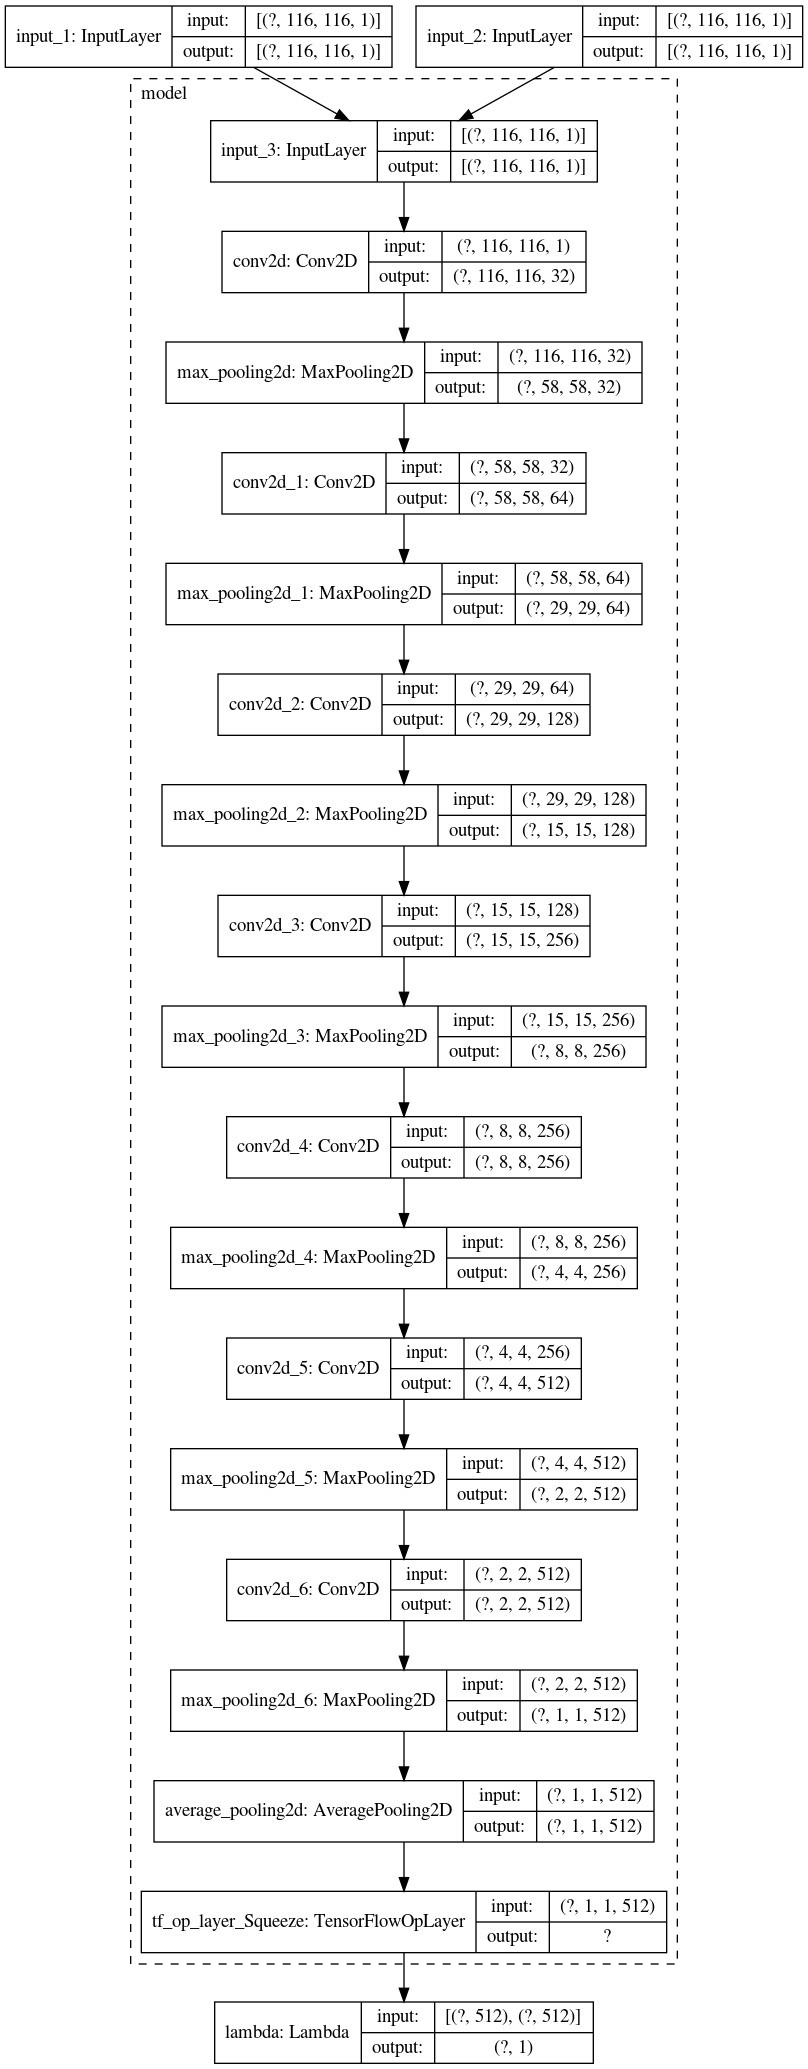
\includegraphics[height=19cm]{figures/model_plot.png}
    \caption{%
        Distance estimation network architecture.
        We have two input images of dimensions $116 \times 116$.
        Each one goes to its CNN (part where we share the weights).
        The output is a scalar value representing the distance between these two images.
    }\label{fig:de-architecture}
\end{figure}
